\chapter{Terminology and Background}
\label{chapter:background}


\chapterprecishere{If you're a baker, making bread, you're a baker. If you make the best bread in the world, you're not an artist, but if you bake the bread in the gallery, you're an artist. So the context makes the difference.\par\raggedleft--- \textup{Marina Abramovic}}
\chapterhung

In this chapter, we introduce terms, elaborate on the already mentioned terms, and discuss the background of our work.
We will use the terms in the way as used in the introduction and also as used by the cited papers, unless we say otherwise.
We will answer the research question:
\rqBackground*

\section{Configuration}

The \intro[execution environment]{execution environment} is information outside the boundaries of each currently running process~\cite{corbato1971multics}.
The operating system introduces these boundaries.
Controlling the execution environment is essential for configuration management~\cite{cons2002pan,huang2015confvalley}, testing~\cite{van2010automating,wang2009context}, and security~\cite{goldberg1996secure,schreuders2012towards,perkins2009automatically,liang2003isolated}.
For our considerations, the most important parts of the execution environment are configuration files, environment variables, and command-line options~\cite{raab2014program}.

An \intro[application programming interface (API)]{application programming interface (API)} defines boundaries on source code level.
Better APIs make the execution environment easier and more uniformly accessible.

\intro[free/libre and open source software]{Free/libre and open source software (FLOSS)}
is software from which the source code can be studied without limitations.
In particular, \intro[FLOSS|see{free/libre and open source software}]{FLOSS} guarantees that source code can be (0) executed, (1) studied, (2) shared, and (3) published with or without modifications~\cite{stallman2002free}.
\intro{FLOSS initiatives}\footnote{We avoid the term FLOSS projects because a project has by its definition a fixed end date.} are communities behind FLOSS.

Modifications in the execution environment change the run-time behavior of \intro[configurable application]{configurable applications}.
We are not aware of any relevant FLOSS application that is not configurable, for example, even ^hello^, ^cat^, and ^echo^ can be configured.

While file systems have APIs with specified behavior since decades~\cite{morgan1984specification,sandberg1985nfs}, access to the execution environment is reimplemented differently within every programming language or even application.\footnote{
With the notable exception of environment variables, where configuration access is standardized.}
Some parts of the execution environment cannot be influenced by other applications after the program has started.\footnote{For example, environment variables and command-line options.}
Other parts of the execution environment can be changed during run-time and as such are subject to \intro[inter-process]{inter-process} communication.\footnote{For example, the file system and shared memory.}

\begin{definition}
\label{def:configuration-setting}
A \intro[configuration setting]{configuration setting},
or \intro[setting|see{configuration setting}]{setting} in short,
fulfills these properties:
\begin{enumerate}
\item
It is provided by the execution environment.
\item
It is \empha[consume]{consumed} by an application.
\item
It consists of a key, a configuration value, and potentially \empha{metadata}.
The \intro{configuration value}, or \intro[value|see{configuration value}]{value} in short, influences the application's behavior.
\item
It can be \empha[produce]{produced} by the maintainer, user, or system administrator of the software.
\end{enumerate}
\end{definition}

A \intro{configuration file} is a file containing configuration settings.
For example, a Web server configuration file includes many configuration settings such as ^port=80^ and ^address=127.0.0.1^.
Their configuration values are ^80^ and ^127.0.0.1^, respectively.
Other information in the configuration file is metadata for the configuration settings (such as comments).
This book is only concerned about configuration settings but not about other forms of configuration.
For example, we configure a computer by assembling its parts, but this is not configuration settings.\footnote{Unless we talk about an application that assembles computers.}

There are different viewpoints of configuration, for example, configuration as activity~\cite{sabin1998product}, decision process~\cite{reiser2009cvm}, or task~\cite{soininen1998towards}.
In this book, we will interface with such activities.
But for us only the result of such activities is of importance, i.\,e., the configuration settings.%
{\parfillskip=0pt plus .8\textwidth \emergencystretch=.5\textwidth \par}

In the literature many synonyms for configuration settings exist.
\intro[user preferences|see{configuration setting}]{User preferences}~\cite{jin2014configurations} and \intro[customization|see{configuration setting}]{customization}~\cite{anderson2002researching} stress that users make the change although that might not always be the case.
\intro[variability point|see{configuration setting}]{Variability points}~\cite{gunther2012software,rhein2016variability,villela2014survey,van2001notion,nadi2014mining,mens2016taxonomy} aim at describing the capability of software to adapt its behavior.
\intro[derivation decision|see{configuration setting}]{Derivation decision}~\cite{software1993reuse,czarnecki2012cool} puts the decisions to make and not the result in focus.
\intro[configuration parameter|see{configuration setting}]{Configuration parameter}~\cite{yin2011empirical,anderson1994towards} is easily confused with other kinds of parameters.
\intro[configuration item|see{configuration setting}]{Configuration item}~\cite{anthony2009context} or \intro[configuration option|see{configuration setting}]{configuration option}~\cite{rabkin2011static,zhang2013automated,zhang2014configuration} are sometimes not applicable, for example, ``proxy option'', or ``language item''.
\intro[configuration data|see{configuration setting}]{Configuration data}~\cite{huang2015confvalley} is often used in the context of programmable gate arrays and has a different meaning in that domain.
We will avoid all these synonyms in the rest of this book, except if we need the term for the distinguished meaning as described here.

From the application's point of view configuration settings are indistinguishable from other input/output data.
What are input/output data for one application, are configuration settings for another application.
\begin{example}
Let us consider a Web server.
The following discussion is only valid from the Web server's perspective, for a browser it would be different.
The Web server's address and port clearly are configuration settings.
Web server requests clearly are not settings.
The contents of the pages delivered are potentially influenced by settings.
Users have server-side settings stored, for example, languages-specific settings.
If the data is stored in cookies, however, it is not a configuration setting because cookies are sent within every request.
In our terminology, Apache's configuration file ^.htaccess^\footnote{It provides configuration files on a per-directory basis.} contains configuration settings even though it is located next to data files.
\end{example}


\subsubsection{Configuration Access}

\intro[configuration access]{Configuration access}
is the part of every software system concerned with fetching and storing configuration settings from and to the execution environment.
There are many ways to access configuration~\cite{kiciman2004discovering,xu2013blame,jin2014configurations}.
\intro[configuration access API]{Configuration access APIs} are APIs that enable configuration access.
Within the source code the \intro[configuration access point]{configuration access points} are configuration access API invocations that return configuration values.

\pagebreak
\begin{example}
\fixtheorem

\begin{code}[language=Cpp]
char * getenv (const char * key);
int main()
{
    getenv ("PATH");
}
\end{code}

The forward declaration on line~1 specifies the configuration access API ^getenv^.
In line~4 we have a configuration access point.
\end{example}

Configuration access happens at various points in time throughout deployment and run-time~\cite{anthony2009context}.
\citet{kang1990feature}~distinguish between compile-time, load-time, and run-time configuration access.
We will use more elaborate distinctions:

\begin{itemize}
\item[]
\begin{description}[font=\textintro]
\item[Implementation-time] configuration accesses \index{implementation-time}
are hard-coded settings in the sou\-rce code repository.
For example, architectural decisions~\cite{zdun2007patterns} lead to impl\-ementation-time settings.
Often developers decide that configuration access shall be postponed, leading to the other points in time below.

\item[Compile-time] configuration accesses \index{compile-time}
are configuration accesses resolved by the build system while compiling the code.
Similar to implementation-time configuration accesses, run-time lookups are not necessary and compilers can optimize away not-executed paths.
Different from implementation-time, the build process also considers the execution environment outside the source code repository.
This technique is often discussed along with software product lines~\cite{mezini2004variability,van2001notion}.
The implementation techniques range from special-purpose programming languages, generated code, and definitions substituted by preprocessors.
Because avoiding complexity in the build system is rarely a pursued goal, the number of such configuration settings can be extremely large in FLOSS~\cite{passos2015feature}.
Nevertheless, these settings are hardly used by non-maintainers because changes require recompilation.
Systems providing compile-time settings usually provide alternatives.
For example, although Linux has many preprocessor directives, loadable kernel modules with parameters\footnote{They were added to Linux in 1995, and around 2000 modules were used everywhere in Linux.} (next to other techniques) enable us to set nearly all configuration settings at later points in time.

\item[Deployment-time] configuration accesses \index{deployment-time}
are configuration accesses while the software is installed.
Techniques that do configuration access solely during deployment are used rarely in FLOSS.
For example, in Debian GNU/Linux the installation procedure of alternative tools changes symbolic links so that the favorite tool is preferred.

\item[Load-time] configuration accesses \index{load-time}
are configuration accesses during the start of applications.
The application accesses the execution environment only while initializing but does not synchronize its in-memory configuration settings with the execution environment later.
For example, accesses to environment variables and command-line options are load-time configuration accesses.%
{\parfillskip=0pt \emergencystretch=.5\textwidth \par}

\item[Run-time] configuration accesses \index{run-time}
are configuration accesses during execution not limited to the startup procedure.
To trigger configuration access at run-time we usually have to notify the application.
Then the application rereads its execution environment and updates its in-memory configuration settings.%
{\parfillskip=0pt \emergencystretch=.5\textwidth \par}
\end{description}
\end{itemize}

We focus on run-time configuration accesses because it is straightforward to avoid configuration accesses to reoccur at a later point of time.\footnote{By ignoring notifications that the configuration settings have been changed.}
Considering run-time configuration accesses in applications that do not support them already, however, usually implies rewriting code.
Furthermore, the user's decision about a configuration value can always be earlier than the point in time the configuration access happens but not vice versa.%
{\parfillskip=0pt \emergencystretch=.5\textwidth \par}




\subsection{Libraries}

\intro[configuration library]{Configuration libraries} provide implementations for a configuration access API.

\subsubsection{Abstractions}

It is an old idea to use an API to abstract from irrelevant details when accessing configuration settings.
The first interface, that is still commonly in use, is ^char *getenv(const^ ^char *name)^.
It was first standardized in 1986 with 4.3BSD and is included in the C89 standard.

The essential operations for configuration libraries are those to get and to set configuration settings in two different ways: \intro{transient} and \intro{persistent}.
The APIs for environment variables only provide transient access, i.\,e., changed configuration settings are lost after restart.
For persistence, \intro[serializer]{serializers} transform the transient data structures to a byte stream to be written into configuration files.
They have other drawbacks in their abstraction, for example, the environment is easily corrupted by directly accessing ^environ^.

Other examples of standard APIs are:
\begin{itemize}
\item ^long pathconf(const char *path, int^ ^name)^,
\item ^long sysconf(int name)^, and
\item ^size_t confstr(int name, char *buf, size_t len)^.
\end{itemize}
These APIs are less generic because they only allow us to request values from a predefined list.
But such APIs are safer:
Typos in the constants to be used for the name are caught by the compiler.


Based on these first steps, the next generation of APIs provided persistence, too.
These libraries usually originated from applications and are often dedicated to special-purpose configuration settings.
This often lead to some specialties, such as function names, that indicate the original application.
For example, ^xf86HandleConfigFile^ parses the ^XF86Config^ configuration file (now called ^xorg.conf^).

Later, FLOSS developers introduced dedicated, general-purpose configuration libraries.
They filled the main gap that was often left by libraries written for specific applications:
They were able to persist configuration files and not only to parse them.
For example, Java Properties and the Universal configuration library parser (^libucl^) are such libraries.

A \intro{configuration source} is an entity containing configuration settings.
For example, configuration files, command-line options and environment variables are configuration sources.%
{\parfillskip=0pt plus .7\textwidth \emergencystretch=.5\textwidth \par}

Another fundamental abstraction introduced by configuration libraries is cascading lookup.
\intro[cascading lookup]{Cascading lookup} allows users to merge different sources of configuration settings in the following way:
If a specific configuration setting is missing in one configuration source, we continue the search in other configuration sources.
For example, cascading lookup was used to \enquote{abstract annotation and XML-based configuration sources}~\cite{nosal2012supporting}.%
{\parfillskip=0pt \emergencystretch=.5\textwidth \par}

Yet another abstraction handles several configuration sources of different configuration file formats in a unified way.
Both the Apache Commons Configuration~\cite{online2016apache} and Zend Config framework~\cite{online2016zend} convert to a common data structure.
The solution of~\citet{poruban2011common,nosal2012supporting} extends this idea by using a meta-model and a declarative translation specification.

\subsubsection{Configuration File Formats}
\label{sec:configuration-file-formats}

At any point during the invention of the abstractions mentioned above, in parallel, developers invented many configuration file formats.
Passwd might be the first configuration file format that has documentation still available\footnote{It was already part of the original UNIX Programmer's Manual \url{http://man.cat-v.org/unix-1st/5/passwd} from \formatdate{3}{11}{1971}.}.
After 10 more years, the number of configuration files suddenly began to explode.
Both UNIX (for example, hosts) and DOS (for example, CONFIG.SYS in DOS 2.0) invented one configuration file format after the other.
In the early history, UNIX preferred comma-separated value (CSV) file formats (for example, next to passwd: fstab, inetd, and crontab) but DOS started with key-value formats.
Then INI got a  popular configuration file format across all operating systems.
\citet{evard1997analysis} evaluated UNIX systems and found 58 important configuration files with up to 45 revisions each (4.6 mean, 2 median).
He says: \enquote{These configuration files are a good area of study because they are relatively simple but can lead to complex issues.}
Later popular configuration file formats include XML~\cite{wadler2003xml}, JSON~\cite{crockford2006json}, and YAML~\cite{ben2005yaml}.%
{\parfillskip=0pt \emergencystretch=.5\textwidth \par}

\intro[semi-structured data]{Semi-structured data}
is a representation of irregular, implicitly-structured data~\cite{abiteboul1997querying}.
In particular, it allows data to be missing, which is not possible in structured data.
It became clear that some forms of semi-structured data are better suitable than others if configuration files are serialized.
\citet{wadler2003xml} describe two properties:
\begin{itemize}

\item[]
\begin{description}[font=\textintro]
\item[Self-describing] \index{self-describing}
means that from the configuration file alone we are able to derive the correct internal representation.

\item[Round-tripping] \index{round-tripping}
means that if a file is serialized and then parsed again, we end up with an identical internal representation.
\end{description}
\end{itemize}

Older formats, such as S-expressions~\cite{mccarthy1960recursive} fulfill these properties.
Many popular formats, such as XML, do \emph{not} possess these properties~\cite{wadler2003xml}.

A property of configuration libraries is the conservation of all metadata found in the configuration files.
Most configuration libraries have limitations in this property.
For example, they do not preserve comments and white spaces.

\label{sec:augeas}
The configuration library Augeas~\cite{lutterkort2008augeas} systematically avoids loss of metadata and ambiguities in round-tripping using lenses.
Lenses are designed in a way that losing information causes extra effort~\cite{foster2008boomerang}.
Furthermore, instead of separating the parser and the serializer, a lens as sole specification is sufficient.
Because lenses are interpreted from up and from down, they are called bidirectional programs.
The current implementation, however, does not provide:
\begin{itemize}
 \item the level of abstraction as often needed because some (structural) properties of configuration files leak through~\cite{berlakovich2016universal},
 \item configuration access APIs for applications since it is only intended to be used by system administrators,
 \item useful error messages on parse errors, and
 \item support for some popular formats such as YAML (type-safe lenses are limited to regular expressions).
\end{itemize}
Despite these limitations lenses are an important puzzle piece to provide support for non-standard legacy configuration files.
Augeas' ability to completely preserve all white spaces is not achieved by other configuration libraries.

Many configuration libraries are already included within the core libraries of programming languages.
For example, Java provides ^java.util.Properties^, and Python has ^ConfigParser^.
Because of the availability, such already included libraries are the most popular ones.
If not included, successful configuration libraries are often specialized to some niche.
For example, ^fontconfig^ allows system administrators to configure available fonts on the system and performs specialized convenience functionality such as font name substitution.

Most likely more configuration file formats than programming languages exist.\footnote{Nearly every programming language can be used as configuration file format.}
Some of them were hyped and then were already forgotten before tools around them matured.
Most of them are unintentional fragmentations, with minor differences such as case sensitivity, key-value separation character, comments\footnote{For example, subversion uses INI with \# instead of ; to start comments.}, and encoding\footnote{For example, Java properties use ISO 8859-1 and Flex properties files use UTF-8 as described in \url{http://help.adobe.com/en_US/FlashPlatform/reference/actionscript/3/mx/resources/IResourceBundle.html}.}.
While these differences are confusing in practice, we will only discuss fundamental differences here.
We will distinguish between document-oriented formats, object-oriented formats, and configuration file formats designed as such.
The distinction must be taken with a grain of salt~\cite{ducharme2004documents}, the concepts behind these different formats are nevertheless useful.

\intro[document-oriented file format]{Document-oriented file formats} are intended to describe complete documents.
These formats provide many structural elements and have a rather heavyweight syntax.
Nevertheless, they are popular for configuration settings.
Strangely, they are hardly used to produce documents even though a literal style is often preferred by system administrators.
One of the rare examples is that in Lynx the configuration file is converted to an HTML page for online documentation.
A typical document-oriented file format is XML~\cite{wadler2003xml}.%
{\parfillskip=0pt \emergencystretch=.5\textwidth \par}

\intro[object-oriented file format]{Object-oriented file formats} are intended to serialize objects from programming languages.
Typical formats include JavaScript Object Notation (JSON) and Object Exchange Model (OEM).
As another example, AIX introduced the Object Data Manager (ODM)~\cite{kar2000managing} for most of its configuration.
ODM allows us to create classes, and their instances are serialized.
S-expressions~\cite{mccarthy1960recursive} and JSON are subsets of programming languages. 
XML can also be used to serialize configuration settings in an object-oriented fashion~\cite{kapolka2002unified}.
Object-oriented file formats seem handy at first but one has to continuously resist to not leak internals, such as names and state, into the configuration files.

Other \intro[configuration file format]{configuration file formats} are formats exclusively designed to contain configuration settings and to be edited by humans.
Earlier representatives are the already mentioned INI, ^XF86Config^, and CSV formats.
For the CSV formats it was soon clear that they are too limited:
The number of keys they can represent is defined by the number of columns.
Thus in newer software like Xinetd, the CSV format was replaced.
In other cases like fstab and crontab, extensions were invented to circumvent limitations.
One trend is to revitalize INI avoiding some of its limitations, for example, as done by systemd or TOML~\cite{papagiannopoulos2015json}.

Some configuration file formats contain code, for example ^sendmail.cf^.
They are harder to comprehend and cannot be edited by programs.
Nevertheless, they are still popular, for example, to configure some window managers.
While all these formats above have many differences, all of them represent configuration settings as \intro[key-value pair]{key-value pairs}~\cite{jin2014configurations,rabkin2011static,xu2013blame,lathia2013open}.
For scripts key-value pairs are the result after execution.
Thus we will, without loss of generality, assume that configuration file formats can be mapped to key-value pairs.




\subsection{Configuration Specification}


\intro[misconfiguration]{Misconfigurations} are configuration settings that cause misbehavior in software~\cite{yin2011empirical,mahajan2002bgp}.
In some situations, misconfiguration becomes manifest because of problematic configuration access, such as wrong transformations~\cite{xu2013blame}.


\intro[configuration specification]{Configuration specification}, or \intro[specification|see{configuration specification}]{specification} in short, describes the behavior and result of configuration access.
Configuration specifications assign \intro[configuration property|see{property}]{configuration properties}, shortened as \intro[property]{properties}, to individual configuration settings.
Properties can be informal, for example, containing documentation, or formal, for example, describing a data type and a transformation rule.
Configuration specification can be internal and external, i.\,e., embedded within the application and in external files, respectively.
External configuration specifications can be written in the same file format as the configuration settings.
Configuration specifications are on a different meta-level than configuration settings.
As shown in \figref{specifications} we separate the universe of all possible configuration specifications into five subsets.

\begin{figure}[htp]
\centering
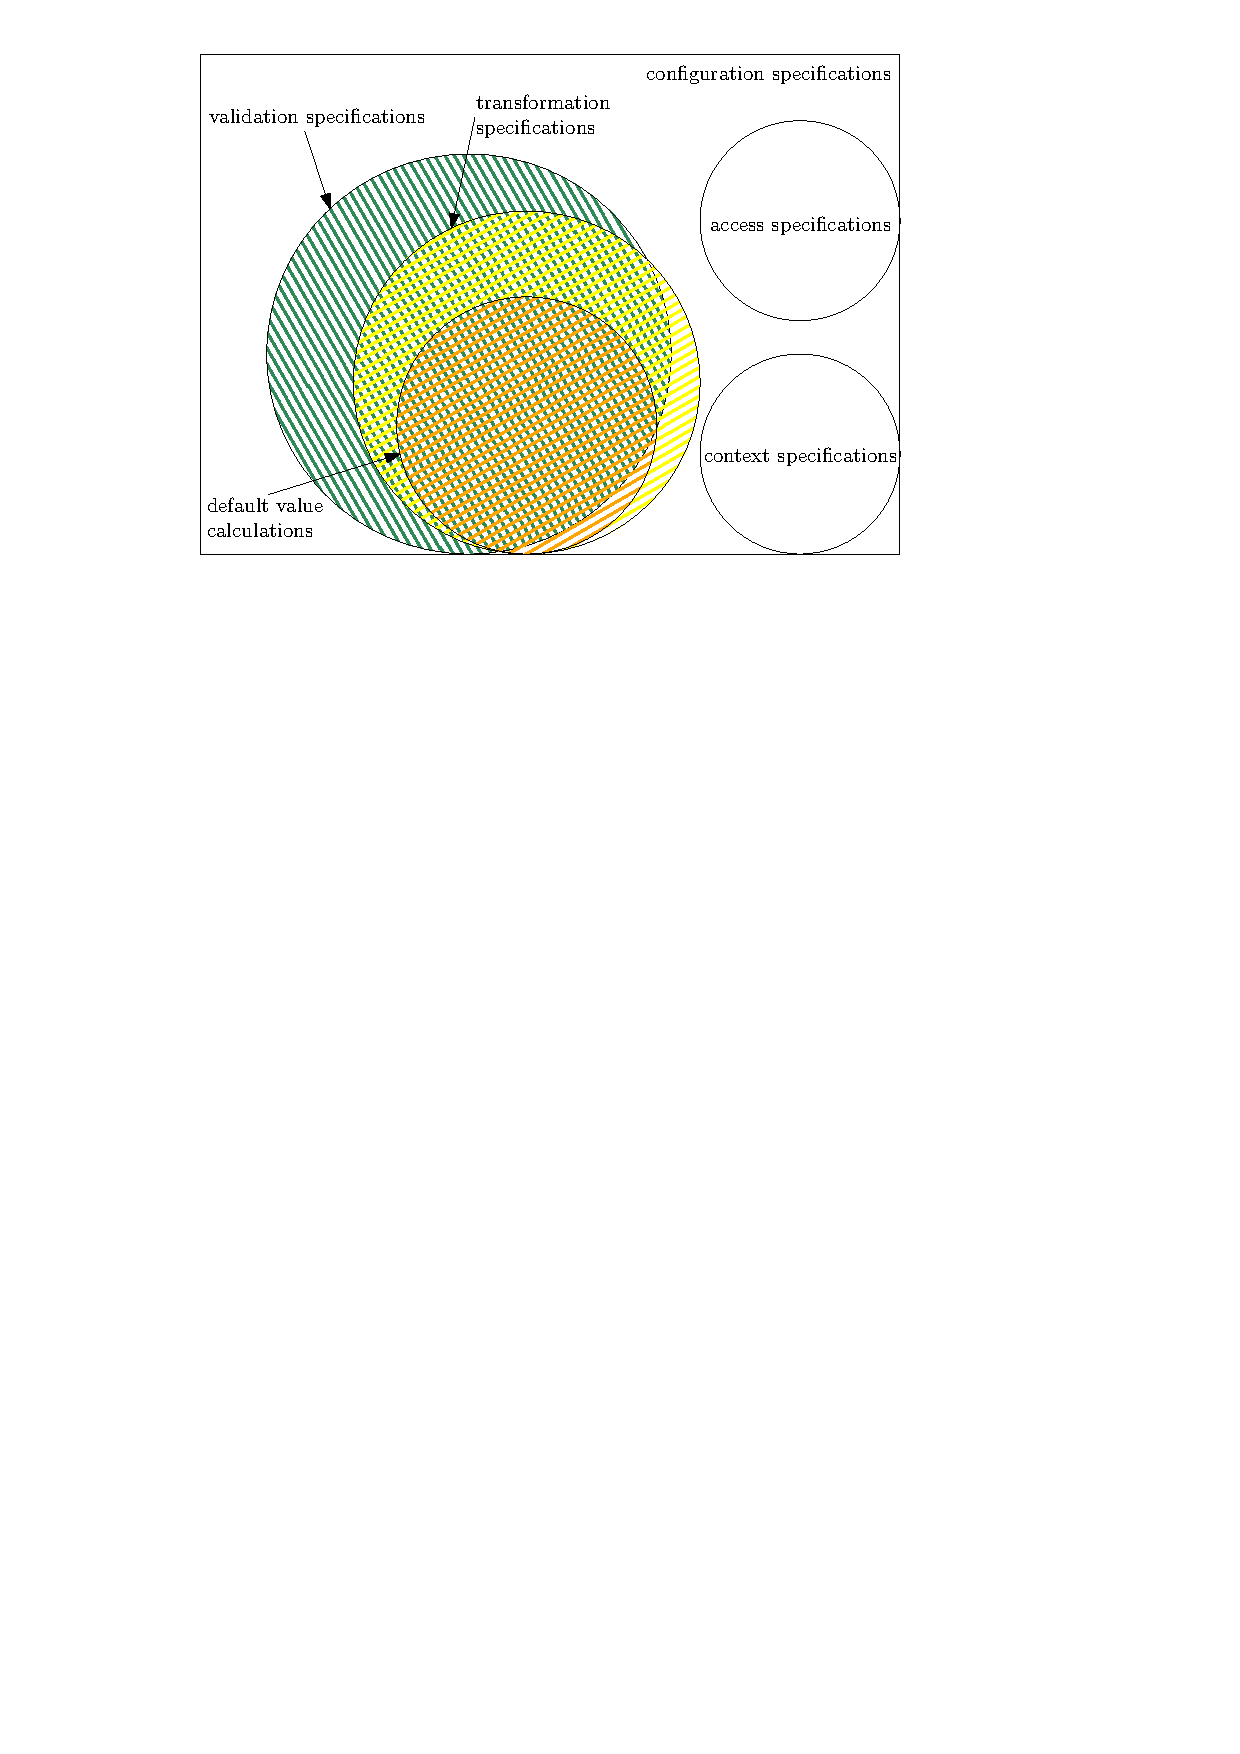
\includegraphics{specifications}
\caption[Types of configuration specifications.]{Types of configuration specifications.
The sizes of the circles suggest the number of language constructs for the different specifications but such numbers vary widely for different configuration specification languages.}
\label{fig:specifications}
\end{figure}

\begin{description}[font=\textintro]
\item[Validation specification] \index{validation specification}
describes all possible valid configuration settings to enable \empha{configuration validation}.
\citet{murata2005taxonomy}~says that validation specifications \enquote{are more precise than those in prose and that we can rely on validators rather than carrying out human inspections}.
Complete validation specifications reject all misconfigurations, and accept all other configuration settings.
Validation specifications are usually incomplete, i.\,e., there exist invalid configuration settings, which do not get rejected~\cite{huang2015confvalley}.
We call source code implementing validation specifications \intro{validation code}.
In other work, validation specification is called \intro[schema]{schema}~\cite{ducharme2004documents,clark2002relax}.
While it is clear that validation specifications shall be checked as early as possible, this is currently rarely achieved.
\citet{xu2016early} wrote a tool to find validation specifications executed too late and aims at pushing configuration validation to the startup of applications.
Ideally, the configuration validation would already happen before the configuration settings are persisted and thus misconfigurations are never present in configuration files.

\item[Transformation specification] \index{transformation specification}
describes how configuration settings shall be transformed.
Because not every transformation accepts arbitrary strings as input most of these specifications are implicitly validation specifications.

\item[Default value calculation] \index{default value calculation}
complements other forms of configuration validation~\cite{eichelberger2013systematic,brummermann2012formalizing}.
While technically a subset of transformation specifications, it has tremendous importance for configuration settings.
Instead of creating a need to synchronously change configuration settings, \intro[default value]{default values} are calculated from other configuration settings.

\item[Access specification] \index{access specification}
describe which configuration file and format shall be used for retrieving configuration settings.

\item[Context specifications] \index{context specification}
are discussed thoroughly in chapters \ref{chapter:approach} to \ref{chapter:backend}; and for the definition see \secref{context-specification}.
\end{description}


\subsection{Configuration Management}
\label{sec:background-configuration-management}

\intro[configuration management]{Configuration Management}
is a discipline in which configuration (in the broader sense) is administered.
Configuration management makes sure computers are assembled from desired parts and the correct applications are installed.
Furthermore, configuration management ensures that the execution environment of installed applications is as required.%
{\parfillskip=0pt plus .7\textwidth \emergencystretch=.5\textwidth \par}

\intro[configuration management tool]{Configuration management tools}
help people involved in configuration management.
Usually, source code describes the desired configuration of the whole managed system.
Then the configuration management tool tries to converge the actual configuration to the desired one~\cite{burgess1995cfengine}

A currently challenging task within configuration management tools is \intro{configuration file manipulation}.
The use of configuration libraries eases this task.
It makes configuration file manipulation more precise and safe.
Because default value calculations influence the configuration settings the applications receive, additionally local introspection of configuration settings is important for configuration management tools.


\subsubsection{System Administrators}

The \intro[system administrator]{system administrator}
is the most important stakeholder within configuration management.
System administrators need to configure every component in a way so that the overall system has desired properties.
This usually implies solving a constraint satisfaction problem~\cite{sabin1998product}.
Higher-level configuration management tools help us find solutions to such constraint satisfaction problems~\cite{cons2002pan,huang2015confvalley}.

System administration research tries to better understand system administrators~\cite{zhang2014configuration}.
The interest of understanding system administrators emerged rather recently~\cite{anderson2002researching,barrett2004field}.
System administration research uses surveys, diary studies, interviews and observations.
\citet{barrett2003system} tried to initiate a workshop at CHI 2003 to draw the attention of the HCI community towards system administration.
The workshop was already dropped in the next year.
Later \citet{haber2007design} repeated an ethnographic field study similar to the one by \citet{barrett2004field}.
In the study of \citet{velasquez2008designing} interviews and a survey were combined.
In interviews, they found that tools used by system administrators varied widely.
One main result of these studies is that system administrators lack tools that have awareness of the context.

Configuration settings are often centered towards the need of developers.
Thus system administrators and end users struggle to understand the consequence of configuration settings.
State-of-the art is that system administrators and developers need to work together tightly, also known as DevOps~\cite{roche2013adopting}.


\subsubsection{History}

One of the first ideas for configuration management was to clone complete machines---often in combination with file synchronization tools like ^rdist^---and then do necessary modifications with scripts or profiles.
\intro[profile]{Profiles} are groups of configuration settings between which the user can easily switch.
This allows us to copy all needed configuration settings onto every machine and afterwards decide which machine is used for which purpose.
While the approach is powerful if all machines are nearly identical, it shows severe limitations once the machines start to differ significantly.
This was state of the art for a long time, until in 1994 when \enquote{the community nearly exploded with four new configuration systems}~\cite{evard1997analysis}:

\begin{description}
\item[lcfg] from~\citet{anderson1994towards}.
The development of lcfg started first in 1991~\cite{anderson1991local,anderson1994towards}.
Nevertheless, its development still continues \cite{anderson2002lcfg,hintsch2016review}.
\item[GeNUAdmin] from~\citet{harlander1994central}.
\item[omniconf] from~\citet{hideyo1994omniconf}.
\item[config] from~\citet{rouillard1994config}.
\end{description}

According to \citet{hintsch2016review}, in 2016 the number of papers published with a configuration management tool in focus is:
15 papers about CFEngine, 11 papers about Puppet, 9 papers about Chef, 7 papers about lcfg, and 3 papers about BCFG2.


\subsection{Context-aware Configuration}


As adapted from~\citet{chalmers2002contextual}:
\begin{quote}
\intro[context]{Context} is the circumstances relevant to the configuration settings of the application.
\end{quote}

We extend the definition with:
\begin{quote}
\intro[context-aware configuration]{Context-aware configurations} are configuration settings that are consistent with its context.
\intro[context-aware configuration access]{Context-aware configuration access} is configuration access providing context-aware configuration.
\end{quote}

Next we investigate the research question:
\rqBackgroundViewpoints*

\subsubsection{Types of Configuration}

\begin{figure}[htp]
\centering
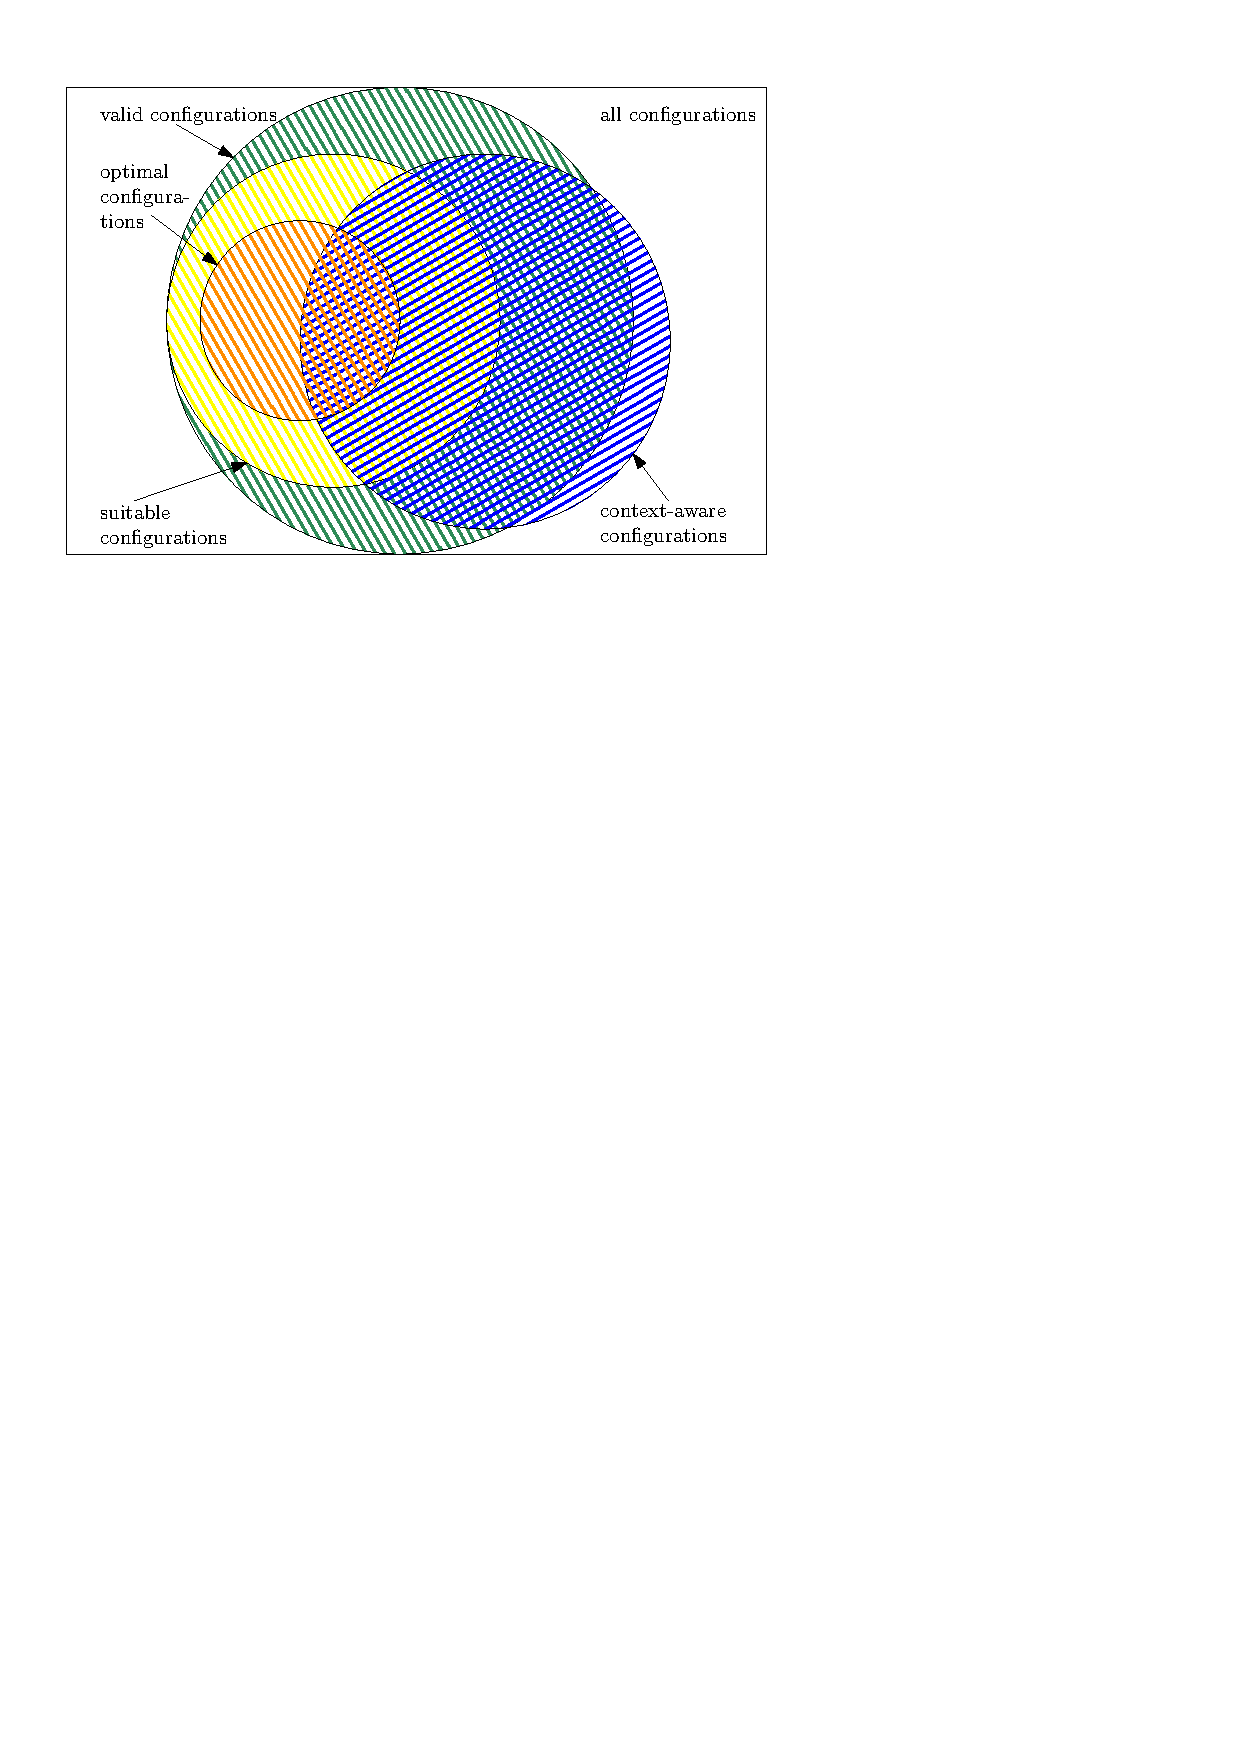
\includegraphics{configurations}
\caption[Types of configurations.]{Types of configurations.
The size of circles does not have a meaning here.}
\label{fig:configurations}
\end{figure}

According to~\citet{wielinga1997configuration} we have three different types of configurations (valid, suitable, and optimal).
We will extend it with a fourth type, orthogonal to all others that we will call context-aware configuration:

\begin{itemize}
\item[]
\begin{description}[font=\textintro]
\item[Valid configuration] \index{valid configuration|boldindex}
does not contradict the present validation specifications.
With a valid configuration, applications can start but they may not do what the user wanted or may be inconsistent with context.

\item[Suitable configuration] \index{suitable configuration|boldindex}
is valid with respect to additional specifications from the user that describe the system the user requires~\cite{kirsch2016requirements}.

\item[Optimal configuration] \index{optimal configuration|boldindex}
is optimal with respect to given optimization criteria.
Optimization criteria are important if managing configuration of many computers but are rarely needed for configuration access discussed in this book.

\item[Context-aware configuration] \index{context-aware configuration|boldindex}
is in accordance with its context.
Unlike configuration settings, the context changes in ways outside of our control.
Context-aware configuration can also be valid, suitable, and optimal.
\end{description}
\end{itemize}


\subsubsection{Viewpoints}


Three \intro[viewpoint]{viewpoints} are important for context-aware configuration:

\begin{description}
\item[Sensors:] \intro[context sensor]{Context sensors} derive context from information sources of the system.
Adding new context sensors increases the context available in a system.
Configuration that was context aware before, can be context unaware with respect to the context acquired from the new context sensors.

\item[Users:] Context awareness can be subjective with respect to the needs of a user.
For different users, we may need different context specifications.
Configuration that is context aware for one user, can be context unaware regarding the wishes of another user.
According to \citet{khalil2005context,khalil2005improving} personalization is essential.

\item[Time:] Because context varies in time, on changes, we need to renew the context awareness of configuration settings.
In such situations we speak of \intro{context changes}~\cite{geihs2009comprehensive,kamina2014context}.
Without renewing configuration settings, configuration settings context aware in one moment of time, can be context unaware in the next moment.
\end{description}

These viewpoints imply that fully context-aware configuration is only possible with a closed-world assumption.
With an open-world assumption, we can always construct differences in the viewpoints that make previously context-aware configurations inappropriate.
Thus it is essential that users have possibilities to personalize and extend context specifications to cope with differences in the viewpoints.

Time and users are not only a viewpoint but can be a context, too.
For example, context sensors can look into the working schedule to change the context according to currently ongoing meetings.

We answer the research question:
\rqBackgroundViewpoints*
\begin{finding}
At least three viewpoints, i.\,e.\ sensors, users, and time, decide about how to interpret the current context.
There may be further viewpoints, too.
\end{finding}





























\section {Configuration Specification Languages}

\intro[configuration specification language]{Configuration specification language}
is a relatively vaguely defined term---it is a language where some kind of configuration is specified.
In this section, we will investigate different kinds of configuration specification languages.

We aim at configuration specification languages that provide background for \elektra{Spec}.
We investigated who already created configuration specification languages to improve configuration access, answering the following research question:
\rqBackgroundSpecificationLanguages*

\begin{hypothesis}[RQ~\ref{rq:background-specification-languages}]
We expect to find a large variety of configuration specification languages that already solve some parts of the configuration integration problem.
\end{hypothesis}

\subsection{Method}

We did a survey of all configuration specification languages as revealed by Google Scholar with the search term:
\begin{verbatim}
language
"configuration specification" OR
"configuration description" OR
"configuration definition" OR
"configuration declaration"
\end{verbatim}

This search yielded several thousand articles.
We grouped them by dates because of download limits:
\begin{verbatim}
1950-1998     946 articles
1999-2004     919 articles
2005-2007     786 articles
2008-2010     872 articles
2011-2012     723 articles
2013-2016     810+ articles
\end{verbatim}

The ^+^ sign means that we subscribed to the search term to keep track of new incoming articles.
We scanned through the titles of all papers---or if this was not enough, we read the abstract---to filter off-topic papers.
In particular, we removed all articles that describe general purpose languages, behavioral descriptions, or that are domain-specific.
After this process, we grouped papers that described the same configuration specification language.
As result, we found 92 configuration specification languages.
Due to lack of time, we only further processed the ones that are at least remotely related to \elektra{Spec} and are of interest for this book.
In this step, we excluded about \sfrac{3}{4} of the configuration specification languages.

In the rest of the section, we will describe four selected properties, i.\,e.\ expressiveness, reasoning, modularity, and reusability, for some configuration specification languages.
Others are mentioned in ``Others''.

\subsection{UML}

\citet{felfernig1999knowledge,felfernig2000uml,felfernig2002joint} describe an approach where the unified modeling language (UML) is used as notation to simplify the construction of a logic-based description.
The papers formally describe the semantics. Tools are available and experimental results show feasibility.

\paragraph*{Expressiveness:}
All UML features, including cardinality, domain-specific stereotypes and OCL-constraints are available.
The basic structure of the system is specified using classes, generalization and aggregation.
Resources impose additional constraints on the possible system structure.
Finally, the require-relation and incompatible-relation allow us to limit valid configurations.

\paragraph*{Reasoning:}
Customers provide additional input data and requirements for the actual variant of the product.
The logical sentences are range-restricted first-order-logic with a set extension and interpreted function symbols.
For decidability, the term-depth is limited to a fixed number.
It is possible to show that the configuration is consistent or that no solution exists.

\paragraph*{Modularity:}
Generalization is present without multiple inheritance with disjunctive semantics, i.\,e., only one of the given subtypes will be instantiated.

\paragraph*{Reusability:}
For shared aggregation additional ports are defined for a part.




\subsection{CFEngine}

CFEngine~\cite{burgess1995cfengine,pandey2012investigating} is a language-based system administration tool that pioneered idempotent behavior.
It uses declarative class-based decision structures.
\citet{burgess2003theory}~introduces theory behind it.

\paragraph*{Expressiveness:}
CFEngine allows us to declare dependences and facilitates some high-level configuration specification constructs.
In its initial variants it neither had validation specifications, cardinalities, nor higher-level relationships.
\paragraph*{Reasoning:}
\notsupported{}
\paragraph*{Modularity:}
\notsupported{}

\paragraph*{Reusability:}
Existing system administrator scripts can be profitably run from CFEngine.


\subsection{NIX}

The NIX language~\cite{dolstra2007purely} claims to be purely functional as a novel feature.
The main concept is the referential transparency both for the configuration specification language and for the system itself.
A large-scale deployment shows that the approach is feasible and practical.

\paragraph*{Expressiveness:}
NIX expressions, for example functions, describe how to build software packages.
The unit of variability is a package.
Additionally, a hierarchical set of properties describes the configuration specification.
Otherwise, the expressiveness is low, NIX describes neither cardinalities nor relationships.

\paragraph*{Reasoning:}
Because of the referential transparency of the system itself, every solution derived from the NIX expressions should be valid, so no reasoning or conflict handling is necessary.
Some operations, however, might lead to a completely new system.

\paragraph*{Modularity:}
The NIX expressions are modular because they ensure absence of side effects and thus can be easily composed.

\paragraph*{Reusability:}
Derivations that describe atomic build actions are reused in other derivations.
Import and inherit features are used to create packages, improving reusability.



\subsection{Pan}

\citet{cons2002pan} invented and used PAN for many machines within CERN.
Furthermore, the language is still used by Quattor.
The configuration database in Pan comprises high-level and low-level descriptions.
The low-level descriptions are in XML syntax.
Here we focus on the declarative, high-level description.

\paragraph*{Expressiveness:}
The Pan language allows users to specify data types, validation with code snippets and constraints.
It only supports lists but no configurable cardinality nor is-a/part-of relationships.
The compiler uses a 5 step process: compilation, execution, insertions-of-defaults, validation, and serialization.

\paragraph*{Reasoning:}
Pan focuses on validating configurations, it is not able to generate new configurations.
Pan provides type enforcement with embedded validation code.

\paragraph*{Modularity:}
The language has user-defined data types (called templates) but otherwise has only minimal support for modularity.
In particular, side effects and assignments hinder modularity of validation code.

\paragraph*{Reusability:}
Reusability and collaboration is only possible via simple include statements and a simple inheritance mechanism of templates.





\subsection{ConfValley}

\citet{huang2015confvalley} introduce systematic validation for cloud services.
ConfValley uses a unified configuration settings representation for tens of different configuration file formats.
Its configuration specification language, called CPL, does not aim to be a type-safe configuration specification language.
It enables, however, system administrators of cloud services to write declarative specifications of properties with correctness constraints.

\paragraph*{Expressiveness:}
CPL introduces many concepts and has non-trivial language features.
Its most expressive elements are first-order quantifiers.
CPL is not able to specify dynamic and complex requirements.

\paragraph*{Reasoning:}
Constraints can be inferred by running an inference engine on configuration settings that are considered good (black-box approach).
Within the validation engine, however, no constraint solver is available.

\paragraph*{Modularity:}
CPL aims at easy grouping of constraints.
Its extensibility has limitations, for example, adding language primitives need modifications in the compiler.
The authors claim, however, that these changes can be done in a straightforward way---at least for predicates.%
{\parfillskip=0pt plus .7\textwidth \emergencystretch=.5\textwidth \par}

\paragraph*{Reusability:}
Using transformations and compositions, predicates can be reused in different contexts.
Also with language constructs like ^let^, specifications can be reused.


\subsection{Others}

\citet{lock2005strider} invented Strider that supports modeling and analysis of complex systems.

\textsc{Proteus}~\cite{tryggeseth1995modelling} shows the tight relation between software configuration management, like Git or Svn, and configuration specification languages.
\textsc{Proteus} combines both worlds in a powerful build system.

ConfSolve~\cite{hewson2011modelling,hewson2012declarative} is a configuration specification language that is translated to a standard constraint programming language called MiniZinc.
Their focus is in finding configurations for machines and not to compute configuration settings.
ConfSolve generates Puppet code for deployment.

Many other configuration specification languages have been found during the survey~\cite{roll2003towards,pandey2012investigating,hill2011modeling,anderson2002lcfg,deliverable1996tina,lujak2015orcas,sommerville1992configuration,giese2012industrial,huang2007system%
,novak2005automatic%Puppet, Quattor,..
,gunther2012software,berger2013survey,magableh2010primitive,friedrich1999consistency}, but they do not provide configuration access specifications for FLOSS applications.

\subsection{Result}

The result of the survey was that we could not find a configuration specification language to be used as basis.
Instead all configuration specification languages we investigated had a different focus, which leads us to our answer of:
\rqBackgroundSpecificationLanguages*

\begin{finding}
We have to reject our hypothesis for \rqref{background-specification-languages}:
We did not find any configuration specification language that supports our goal of solving the configuration integration problem.
Instead earlier work had at least one of the following two assumptions:
\begin{itemize}
\item Configuration access in applications needs to be used as given.
Configuration management tools have this assumption.
\item Applications need to be reimplemented using new development methods.
Architecture description languages, software product lines, and similar approaches have this assumption.
\end{itemize}
\end{finding}
\par
Both assumptions hinder progress in fixing the configuration integration problem.



















\section{Programming Paradigms}

In this book we will extend from several existing programming paradigms.
This section explains the necessary foundations.


\subsection{Data-driven Programming}

Data-driven programming is a very popular programming paradigm available in most programming languages.
\citet{raymond2003art}~says that \enquote{in data-driven programming, the data [\ldots] defines the control flow of the program. Where the primary concern in OO [object-oriented programming] is encapsulation, the primary concern in data-driven programming is writing as little fixed code as possible. Unix has a stronger tradition of data-driven programming}.
\citet{raymond2003art}~further elaborates \enquote{Lisp and Java programmers call this introspection; in some other object-oriented languages it’s called metaclass hacking.}
We will use the terminology from Lisp and Java and will call the facilities for applications to look up configuration settings and specifications \intro{introspection}.

\subsection{Object-oriented Programming}

Simula is believed to be the immediate ancestor of object-oriented programming~\cite{rentsch1982object}.
Smalltalk further evolved the paradigm~\cite{nierstrasz1987object}.
In homogeneous designs the premise of ``everything is an object'' goes quite far, next to primitive types and classes, even expressions are objects.
But the premise needs to be broken at some level, for example messages normally cannot be objects we can send messages to~\cite{nierstrasz1987object}.
But particularly the sending of messages is central to the object-oriented programming mechanism.

There are different reasons why object-oriented programming got popular.
While first the immediate code-reuse, for example via inheritance, rose to prominence, it soon became clear that subtyping is even more powerful on large-scale systems.
A long-standing problem was nominal versus structural subtyping.
\citet{malayeri2008integrating} found a solution to combine both ways of subtyping.
Object-oriented programming has all building blocks for design patterns~\cite{gamma1994design}.
Sometimes, subtyping even presents elegant solutions for problems that were thought to be intractable~\cite{wang2016expression}.

For details on how to implement an object-oriented system, we refer to \citet{schwartzbach1994object}.
For configuration libraries, object-oriented programming had little impact for two reasons:
\begin{itemize}
\item
Encapsulation has little use in a scenario without behavioral specifications.
Classes exclusively consisting of trivial getter and setter methods have no advantage to directly accessing data.
\item
Subtyping is hardly used in configuration settings.
The reasons are similar:
The benefit of subtyping on simple data types is limited compared to subtyping on objects with behavior.
\end{itemize}

\subsection{Persistence in Object-oriented Programming}


The main limitations of persistence in object-oriented programming is figuratively described as \enquote{Fitting Round Objects Into Square Databases}~\cite{tsichritzis1988fitting}.
Databases and configuration libraries emphasize data independence, which is different from the focus of object-oriented programming~\cite{tsichritzis1988fitting}.
\intro[data independence]{Data independence} aims at separation of the persistent data and their applications using it.

Objects in Smalltalk are persistent, which can be used as replacement for configuration settings from the developer's point of view.
Later systems provided dedicated object serialization~\cite{hericko2003object}.
While it is a good idea to have the persistence format decoupled from objects, efforts usually do not go far enough to have a serialization that fulfills all desired properties for configuration settings.
The fundamental problem is that objects are coherent with the implementation design, which usually has nothing to do with the system administrator's needs.

\subsection{Aspect-oriented Programming}

While \intro[core concern]{core concerns} are the functionality software was designed and modularized for, \intro[cross-cutting concern]{cross-cutting concerns} are usually scattered throughout the code base.
Typical examples for cross-cutting concerns are persistence and logging, both relevant for configuration access.%
{\parfillskip=0pt plus .7\textwidth \emergencystretch=.5\textwidth \par}

\citet{kiczales1997aspect}~suggested to weave separately implemented modules (the cross-cutting concerns) into the main module (the core concern).
After the first implementations for Lisp and Java, other implementations, for example, for C++~\cite{apel2005featurec++}, followed.
While it is straightforward to show that aspect-oriented programming improves modularity, there is doubt if aspect-oriented programming increases development speed~\cite{hanenberg2009aspect} or has advantages during maintenance~\cite{endrikat2011aspect}.

\citet{chiba2012we} proposed a radically different approach:
Instead of extending syntax, they suggested a synchronous copy and paste.
To do so, they remember all concerns in a tree.
This approach allows us to handle cross-cutting concerns over documentation and other non-code artifacts.

Immensely successful (and without alternative) got aspect-oriented programming in system-level tracing frameworks.
For example, DTrace and SystemTap allow system administrators to collect data about the running system.

\subsection{Feature-oriented Programming}

\intro[feature-oriented domain analysis]{Feature-oriented Domain Analysis} (FODA) pioneered methods to reuse requirements~\cite{kang1990feature}.
It distinguishes between compile-time, load-time, and run-time features.

\lstDeleteShortInline^
Mostly unrelated but with the same goals, \empha{feature-oriented programming} emerged.
Feature-oriented programming or software product lines is an appropriate technique to implement program families~\cite{lee2002concepts,van2001notion,midtgaard2014systematic}.
\citet{prehofer1997feature} described them to be similar to (abstract) subclasses or mixins.
Instead of rigid class structure, features are composed when creating objects.
The central problem of \empha{feature interaction} is resolved by \empha{lifting} function of one feature to the context of another.
The basic idea is that only \enquote{a quadratic number of $\binom{n}{2} = \frac{n^2 - n} 2$ of lifters, but an exponential number $\binom{n}{k}, k=1,...,n$ of different feature combinations can be created.}~\cite{prehofer1997feature}
\lstMakeShortInline[postbreak=,keywordstyle={}]^

\citet{apel2005featurec++}~extended the approach with multiple inheritance and templates.
Furthermore, they integrated aspect-oriented features.
\citet{thuem2014featureide}~created a framework based on Eclipse used for educational purposes.
Different from previously mentioned solutions it embeds the feature-oriented domain analysis.

\citet{batory2003tutorial}~gives a short introduction on product lines, which is a design methodology and tool for program synthesis.
The idea is to specify products via features, as done in non-software products such as assembled personal computers.
Such a specification contains programs as constants, and feature refinements as functions with a feature-augmented program as return value.
These constants and functions define a relational algebra.
It is possible to synthesize non-code artifacts or product lines of product families.

\subsection{Subject-oriented Programming}

\citet{harrison1993subject}~coined the term \empha{subject-oriented programming} in order to bring awareness that real-world objects cannot be objectively described.
This would assume that all attributes are intrinsic and not depending on their relation to other objects.
The authors introduced a new paradigm that allows us to describe subjectivity.
For example, a tree has some intrinsic properties, such as its mass and height.
But for most applications, we are interested in subjective, extrinsic properties.
The extrinsic properties are viewpoints about different perceptions of the object.
For example, a woodman wants to compute a sale price and a squirrel wants to compute the food value of a tree.
For subjects only object identity is shared.

\citet{ossher1999using} added lifetime features for subjects, including traceability.
They mainly see benefits of subject-oriented programming for programs in the large.
They claim that within subject-oriented programming design patterns can be implemented as subjects, thus separating code to which they apply.














\section {Context}

Context is a natural thing, at least for humans.
It creates more conversational bandwidth and contributes more bits of information to communication.
As downside, we miserably fail in understanding the message if we do not put enough attention on the context.
In this section, we look at challenges and discuss techniques that tackle the challenges.%
{\parfillskip=0pt \emergencystretch=.5\textwidth \par}

\subsection{Context-aware Applications}

In the last years the shape of computers changed radically.
They often fit into our pocket or even glasses and are fully packed with sensors.
This gives many opportunities to take more context into account.

\intro[context awareness]{Context awareness}
aims to give users the impression of applications and devices to be smart~\cite{raab2015global}.
We want applications to react according to properties of their physical environments.
For example, when an application notices that the device is on battery, energy savings should be given priority.
In the same way, if a tool tells the system administrator that the Web server's and the firewall's configuration settings are inconsistent, the tool is more context aware.
The increased context awareness implies that the relationship between the Web server and the firewall is known to the tool.

Most software has at least some context awareness but often without any explicit consideration in the program design.
Thus it is implemented in the same way as other features are, interwoven in the core concerns.
For others applications, context was an important design goal~\cite{baldauf2007survey}.
\citet{riva2006unearthing} searched for design patterns in code that support context awareness in software.


\subsubsection{Context-oriented Programming}

One of the many systematic ways to write context-aware applications is called \intro[context-oriented programming]{context-oriented programming}~\cite{baldauf2007survey,hong2009context,alegre2016engineering,kamina2014context,dey2000towards,keays2003context,tanter2008contextvalues,schippers2010contextoperational,wasty2010contextlua,appeltauer2009contextcomparision,plaice2010contextcartesian,costanza2006efficientlayeractivation,lowis2007contextbeyond,appeltauer2008dedicated,salvaneschi2012context,hirschfeld2014visibility,springer2016cop,gonzalez2011subjective,aotani2014unifying}.
Contrary to other techniques to improve context awareness, it focuses on the language level.
Its run-time system is rather small, it does not need sophisticated frameworks, databases, or middleware.
Context-oriented programming supports implementation of context-aware applications.

\citet{gassanenko1993context,gassanenko1998context} provided the first implementation using the name context-oriented programming in Forth.
In response to this first work, \citet{costanza2006efficientlayeractivation}~criticized that Forth did not have object-oriented programming concepts.
According to \citeauthor{costanza2006efficientlayeractivation} it is \enquote{not clear whether Gassanenko’s contexts must be fully defined or can be partial and combinable}.
Later context-oriented programming languages extended from object-oriented and often aspect-oriented programming.
For example, \citet{tanter2006context}~combined context awareness and aspects.

Context-oriented programming is a modularization technique on programming language level~\cite{appeltauer2008dedicated}.
So instead of having ^if^ conditions spread within the core concerns of the application, context-oriented programming allows us to separate code for different contexts~\cite{dey2000towards,salvaneschi2012context,schippers2010contextoperational}.
Improving on previous paradigms, context is multi-dimensional and dynamically changed as needed.

The \intro[layer]{layer} is the main concept of context-oriented programming.
Each layer represents a part of the context, and together they compose the context awareness of the application.
\intro[layer!activation]{Activation} and \intro[layer!deactivation]{deactivation} of layers dynamically adapt the application to a new context.
The \intro[layer switch]{layer switch} is the response for context changes:
They imply activations or deactivations of the layer as needed by the context.
Information about currently active layers is usually stored in a data structure.
Layers naturally cut across the whole system and provide a natural modularization concept~\cite{appeltauer2009contextcomparision}.
Context-oriented programming has no restrictions on when layer switches occur.
This dynamic behavior poses challenges related to efficiency~\cite{raab2015global,appeltauer2009contextcomparision}:


\begin{enumerate}
\item Activation and deactivation of layers can be inefficient.
\item Execution time, even without any layer switches, can be problematic.
\end{enumerate}

For both problems, improvements were suggested:
For layer activation \citet{costanza2006efficientlayeractivation} build upon heavily optimized language features.
\citet{bockisch2006efficientcontrolflow} employed control flow pointcuts in a virtual machine.
Despite these optimizations, \citet{appeltauer2009contextcomparision} revealed that performance penalties of \p{75} to \p{99} are common~\cite{raab2015global}.


\intro[context-oriented software engineering]{Context-oriented software engineering} facilitates a \enquote{methodology that guides us to a specification of context-dependent requirements} and a \enquote{methodology to systematically organize context-dependent requirements.}~\cite{kamina2014context}.
One of the hypotheses underlying context-oriented software engineering is: \enquote{The factors dynamically changing the system behavior are candidates for contexts.}
Context engineers derive a design model on the basis of a requirements model.
It provides a systematic mapping from context-dependent use cases to layers~\cite{kamina2014context}.


\subsection{Contextual Values}


\citet{tanter2008contextvalues} introduced a lightweight extension to context-oriented programming:
\intro[contextual value]{Contextual values} are variables whose values depend on the context in which they are read and modified.
They \enquote{boil down to a trivial generalization of the idea of thread-local values}.
The key idea is to use layers as \enquote{discriminate amongst possible values, not only the current thread}~\cite{tanter2008contextvalues}.
Side effects are limited to the respective context~\cite{raab2016unanticipated}.
Furthermore, contextual values naturally work along with layers as introduced in context-oriented programming.%
{\parfillskip=0pt plus .7\textwidth \emergencystretch=.5\textwidth \par}

The semantics of contextual values are like variables, but their observed values change according to the context.
When reading a contextual value within a different context, the value can be different even though no assignment occurred.
When writing to a contextual value, the written value is only visible within the current context that allows us to limit the contextual value's scope.
